% Chapter 6

\chapter{Experimental Protocol} % Main chapter title

\label{Chapter6} % For referencing the chapter elsewhere, use \ref{Chapter1} 

\lhead{Chapter 6. \emph{Experimental Protocol}}

%----------------------------------------------------------------------------------------

The experimental protocol was designed around the nine experimental requirements presented in Subsection \ref{expreq} and corresponding to the four research hypotheses introduced in Section \ref{reshypo}. \\
When starting the project, I found out that the planning I had introduced in Section \ref{propla} could not work: the reward function requirement (E1) cannot be worked on before the DQN implementation (E4) and the DDPG implementation (E6), because the reward function may depend on the controller implementation and outputs. Furthermore, because the DQN controller outputs discrete actions and the DDPG controller outputs continuous actions, they would require different reward functions. The new plan was thus to start with the second experimental requirement E2 (implementing the wall following controller), then assess it (E3) and then implement and train the Deep Q-Network controller (E4), defining the reward function at the same time (E1). I would then do the same with the DDPG controller and finish with the Sim2Real gap assessment (E8) and the overall conclusions (E9). \\
As explained in Section \ref{reshypo}, the DQN and DDPG controllers would be trained on the ``RedBull Ring" racetrack from \cite{bosello} for requirements E4 and E6. The assessment of all three controllers in the simulator (wall follower, DQN and DDPG) would then be done on the RedBull track as well as the Silverstone (Appendix \ref{silverstone}) and Monaco (Appendix \ref{monaco}) racetracks. Those tracks are scaled to one-tenth of their actual size to be at the same scale as the car. \\
Those specific tracks were chosen for several reasons. Firstly I thought the Red Bull Ring track to be a good training map because it presents most of the challenges that the controller will encounter on other racetracks: a sharp turn (n°3 Remus, see Appendix \ref{redbull}), wide turns (6,7) and two long straight lines, all of that on a very short circuit, which I think makes for good training data. The second track, Silverstone, is much longer with very long curves and some chicanes, which represents a different challenge: many small adjustments in the long curves and swift adjustments for the chicanes. The Monaco track also offers a different challenge, with many hairpin turns (5,6 and 16, see Appendix \ref{monaco}). \\
\section{Modifications to the experimental requirements}
After trying to implement the DDPG controller, I decided to drop experimental requirements E6 (Implement and train DDPG) and E7 (DDPG assessment). I had previously reviewed a DDPG implementation suitable for autonomous racing (\cite{Reference4}), but I found it too time-consuming to make it work alongside the F1Tenth simulator. Furthermore, the number of hyper-parameters of the DQN controller made it very time-consuming to complete experimental requirement E4 (6 different DQN controllers had to be trained for a total of 24 DQN assessments on all racetracks). I had assigned a lower priority to the DDPG requirements, and dropping them was considered not to be too detrimental to the overall dissertation because the results from the Wall Following and DQN controllers were sufficient to answer research hypotheses 1, 2, 3 and 4. \\
After some consideration, I decided to also assess the controllers (experimental requirements E3 and E5) on a fourth track (see Appendix \ref{oval}). This track has a very simple oval shape, which makes it easy to reproduce in real life using flexible tubing; this would make the Sim2Real gap assessment (experimental requirement E8) much more meaningful because the metrics introduced in Section \ref{eva} would be comparable on a whole lap of the track and not just on a small portion of it. I defined the shape of the track to make it as compact as possible but with a sufficient track width. \\
\section{GitHub repository}
The GitHub repository is structured with folders for each controller, a folder for the F1Tenth simulator, one for the experimental results as Excel files, and one for the Latex code of this dissertation. Several Readme files have been written to explain the procedures and parameters for each experiment. \\
The \verb|EXPERIMENT_PARAMETERS.md| file explains in detail the process I followed to set up the controllers with the F1Tenth simulator. I found it very important to use the 2.0.0 version of the Tensorflow library; this was quite challenging on my laptop as my CPU uses the ARM architecture, and there is no easy way to install the TensorFlow library on an ARM processor. After asking on StackOverflow, I was advised to use the pre-built binary available at \url{https://github.com/PINTO0309/Tensorflow-bin#usage}, which is built for the Raspbian Linux distro but also works on Ubuntu 20.04.3. 

\section{Wall Following implementation}
The second experimental requirement (E2) was to implement and tune the wall following controller in the simulator. My implementation is based on the code shown in the official F1Tenth labs and uses the equations introduced in Subsection \ref{walllidar}. \\
The tuning of the PID controller was done manually as follows: first, I set the three gains $k_p$, $k_d$ and $k_i$ to zero. Then, I increased $k_p$ until the response to a disturbance was a steady oscillation; I then increased $k_d$ until no oscillations were left. I then repeated steps 2 and 3 until $k_d$ didn't stop the response from oscillating. I finally increased $k_i$ until the response reached the set point within only two oscillations. This last step is a compromise between speed and accuracy: if $k_i$ is too small, the controller will be very fast but will overshoot the angle, and if it is too big, the car will react much slower. More information about the process and the parameters can be found on the project's GitHub at \url{https://github.com/HL-Boisvert/MSc_Project_HW}. \\
Once E2 was completed, I had to gather the experimental values for E3. I decided to export the data to a .csv file, which can then be processed in Excel. This was done using the Python \verb|csv| package, which offers much flexibility for exporting the ROS data to .csv format. The export script is implemented as a Python class, instantiated by the WallFollow class. 

\section{Deep Q-Network implementation}
The Deep Q-Network controller used to obtain experimental results is extensively based on the implementation from \cite{bosello}. I will first explain the code's architecture and then introduce the differences I've made to the original code. \\
The UML diagram of the final code is introduced in Figure \ref{uml}.
\begin{figure}
\centering
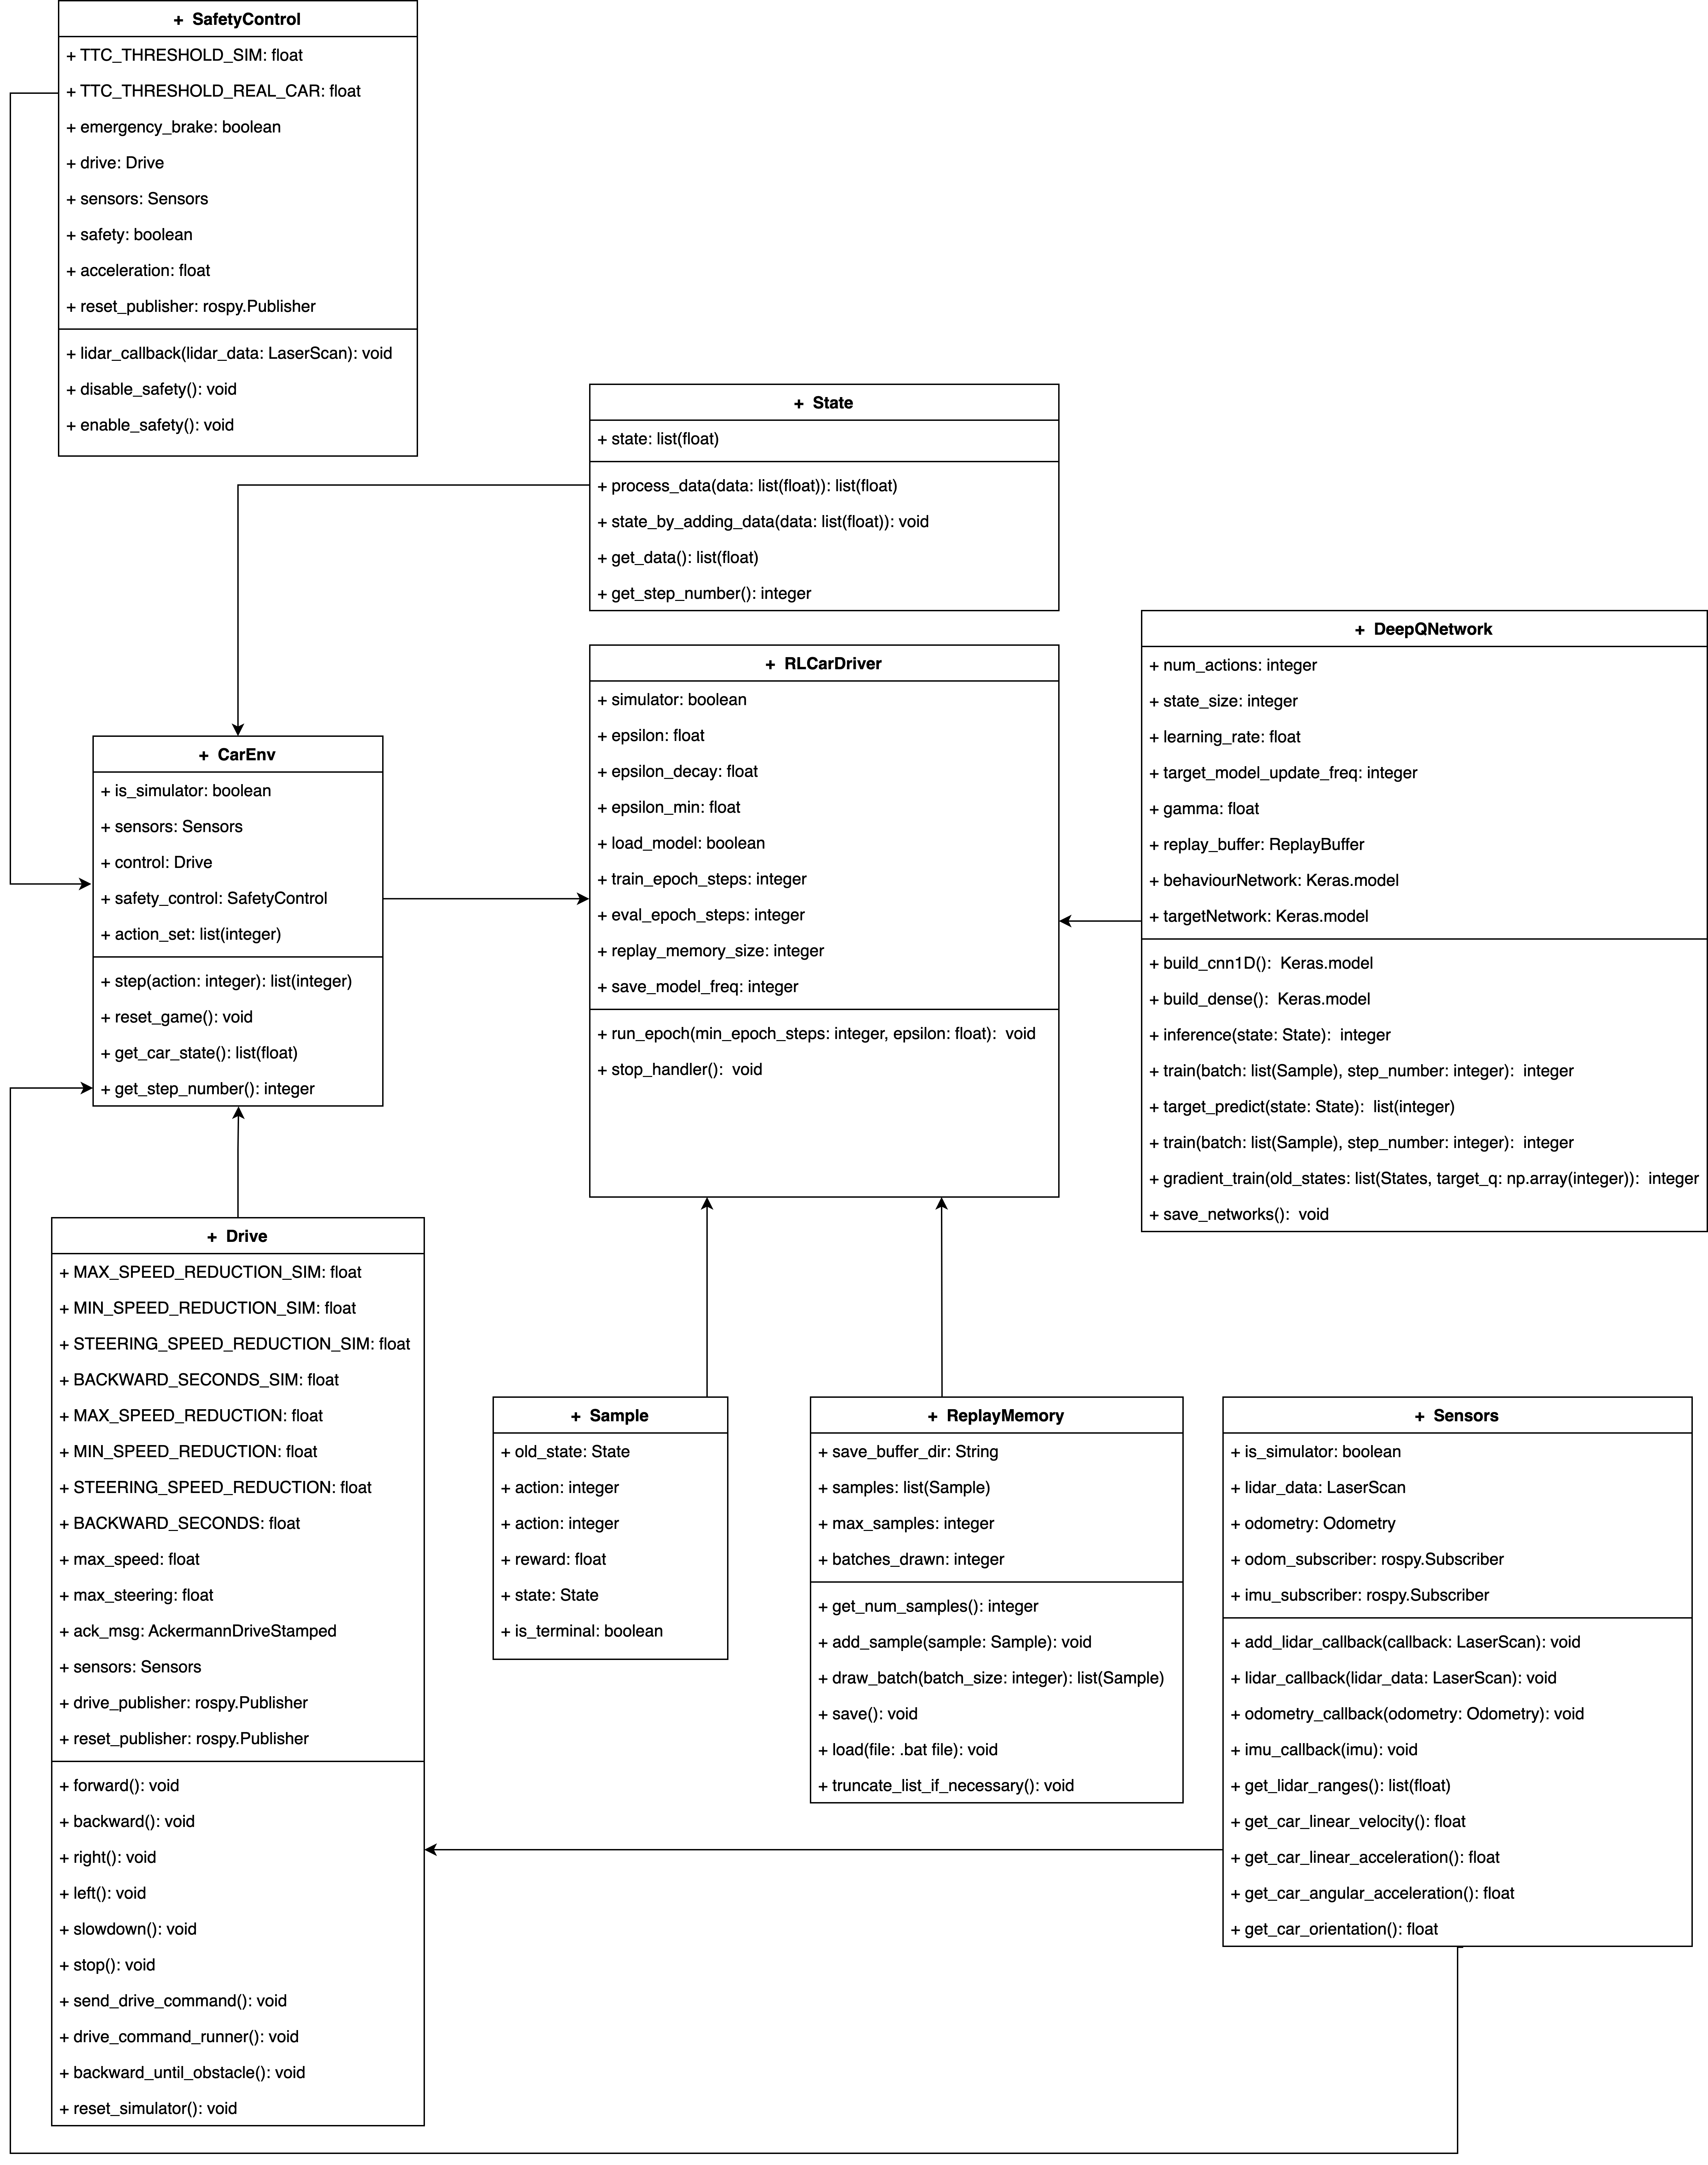
\includegraphics[scale=0.12]{Figures/UML_diagram.png}
\caption{UML diagram of the Deep Q-Network implementation based on \cite{bosello})}
\label{uml}
\end{figure}

The code is structured around three main classes: \verb|RLCarDriver|, \verb|CarEnv| and \\ \verb|DeepQNetwork|.	\\
The \verb |RLCarDriver| class is responsible for three things: setting up the output and logging directory, parsing the parameters from the user input and running the \verb |run_epoch()| function inside of a \verb |while(not stop)| loop. The \verb|run_epoch()| function does several things. First, it gets the state from the environment, then updates the value of epsilon; it then computes the action of the agent according to the epsilon-greedy policy, calling the \verb|DeepQNetwork| class if necessary; finally, it makes a move, and records the experience in the replay memory. \\
The \verb |CarEnv| class is the interface which enables communication between the F1Tenth simulator and the controller; it instantiates the \verb|State|, \verb|Drive|, \verb|Sensors| and \\ 
\verb|SafetyControl| classes. The \verb|Drive| class publishes the Ackermann messages to the \verb|\drive| topic, according to the action sent by the CarEnv class (see Figure \ref{inputs_outputs}). The Sensors class subscribes to the \verb|\odom| and \verb|\scan| topics for them to be stored in a state: the \verb|State| class stores the LiDAR distance values as well as the speed of the agent. \\
The \verb|SafetyControl| class has not been modified from \cite{bosello} and sends the \verb|stop| action to the \verb|Drive| class if the car gets too close to an obstacle. \\
The \verb|DeepQNetwork| class implements the actual DQN algorithm. It creates the behaviour and target NNs and defines a training step according to the pseudo-code introduced in Subsection \ref{dql}. It takes as an input the LiDAR and velocity data from a specific state stored in the Replay Memory as a sample and outputs an integer representing an action (like going forward or turning left) through the \verb|inference(state)| function. \\
The subscribers, publishers and topics are shown in Figure \ref{pub_sub}.
\begin{figure}
\centering
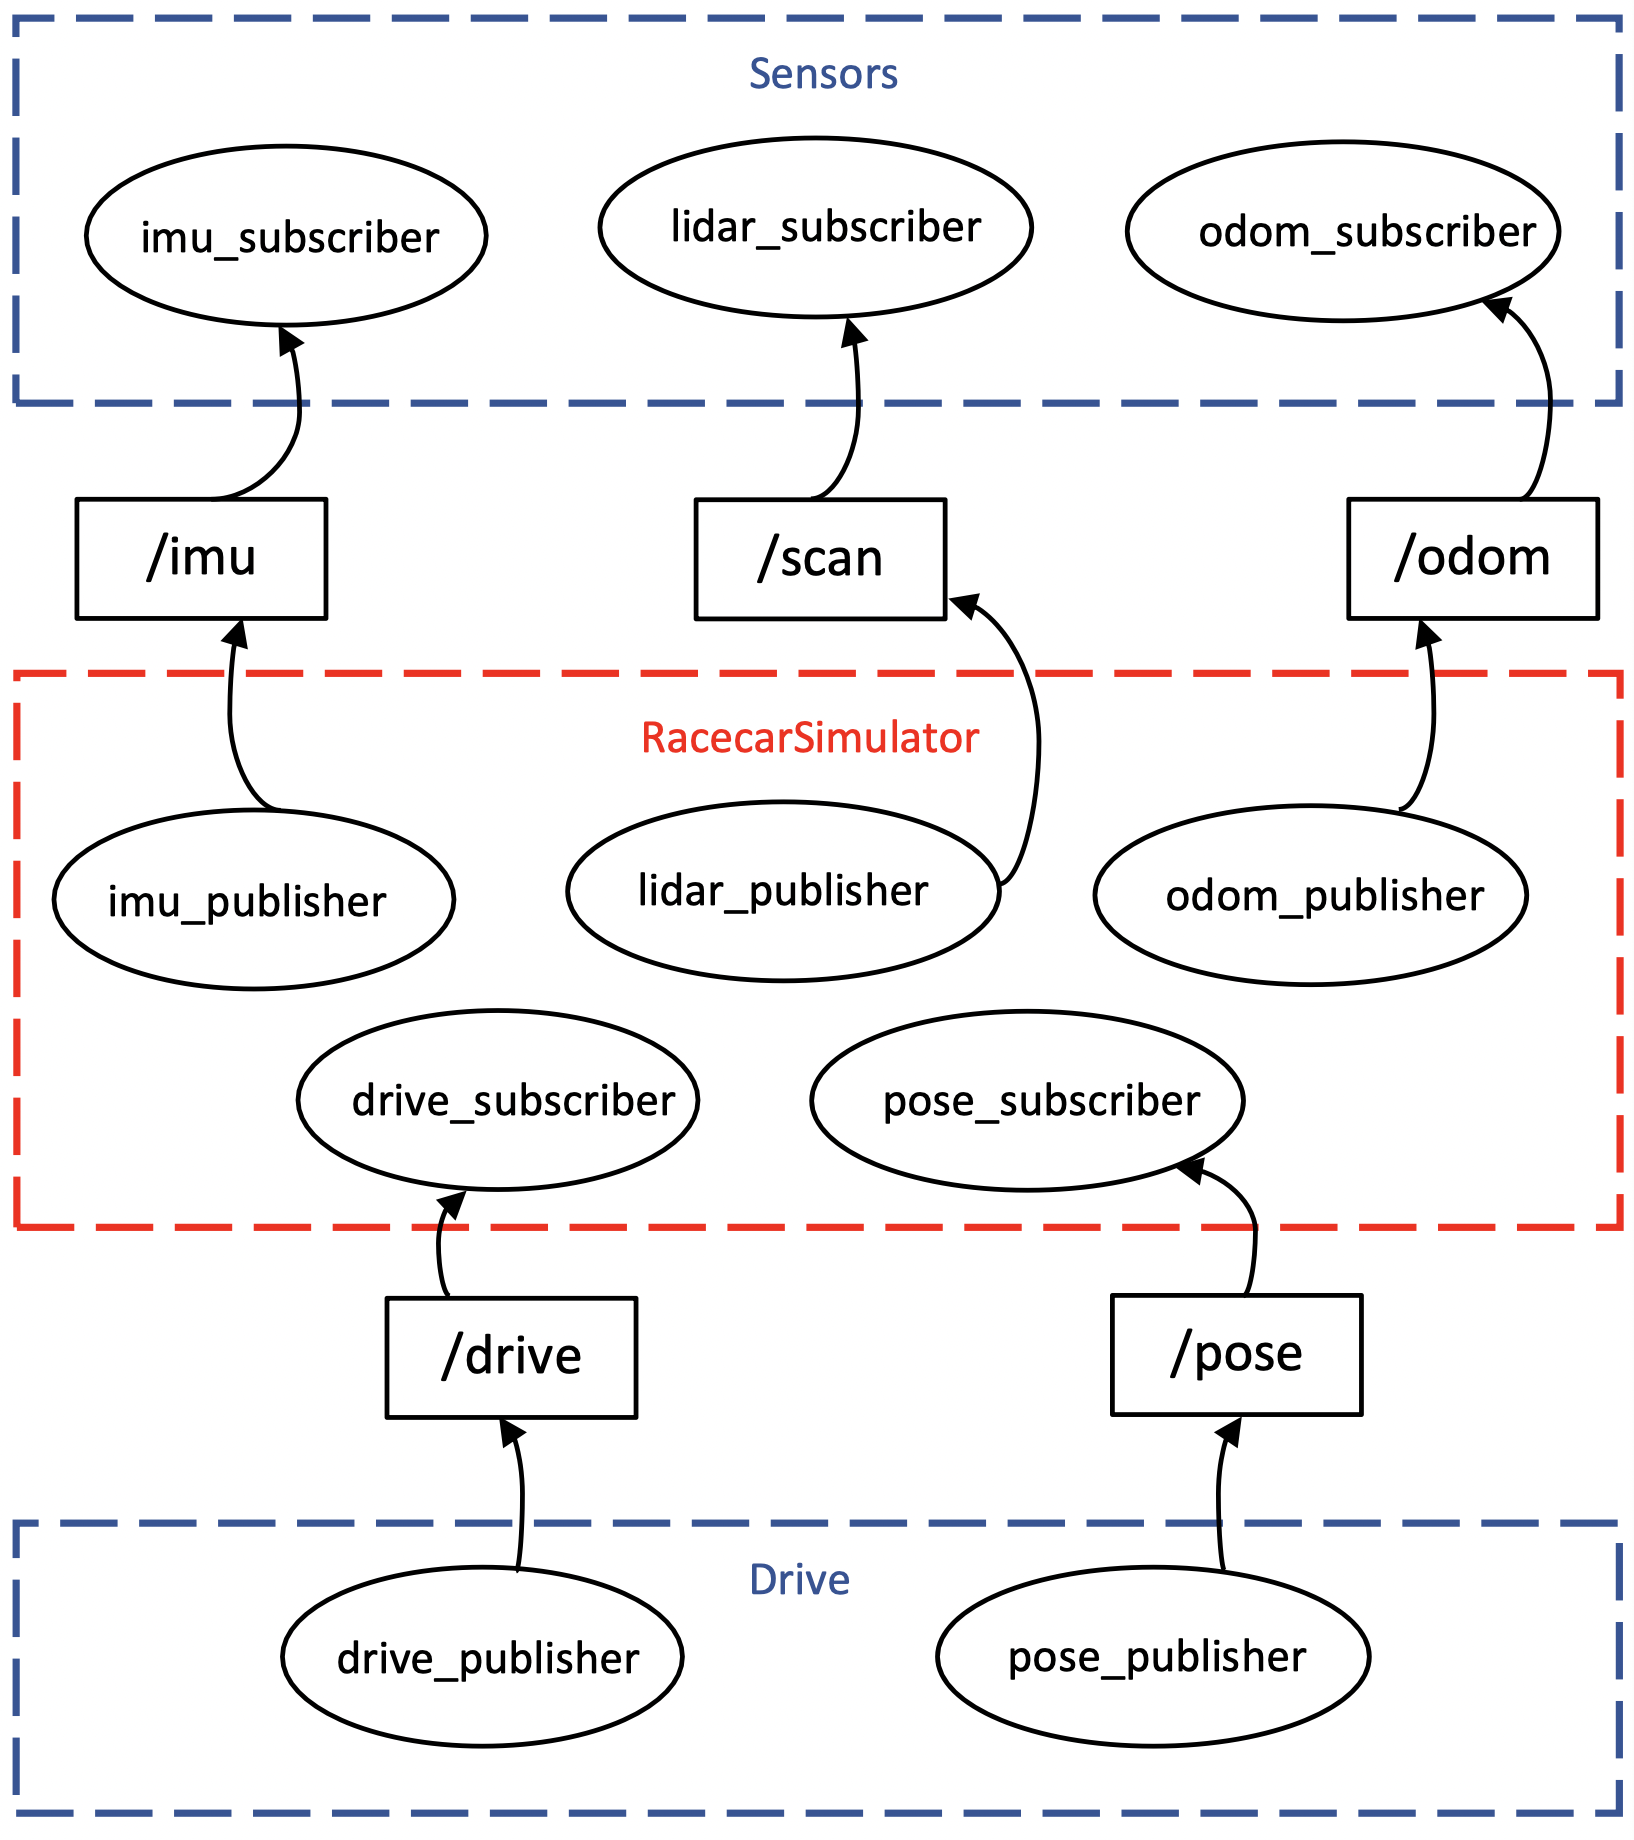
\includegraphics[scale=0.33]{Figures/pub_sub.png}
\caption{Subscribers, publishers and topics for the Deep Q-Network implementation}
\label{pub_sub}
\end{figure}

I have made several changes to the implementation from \cite{bosello}: I've added a class for exporting data to CSV format to then use it in Excel; I've made it possible to choose between different reward functions; I've made the saving and loading of a trained network more straightforward, and I've removed several parameters and classes that were not needed for the experiments.
\section{Reward functions}
The first requirement (E1) was to define a reward function that incentivises a safe, smooth and fast control of the car. Several reward functions were considered for the DQN controller. \\
Before defining the reward function, I had to define the actions that the RL agent would be able to perform. The controller can send two types of commands to the agent through an AckermannDrive Message: a desired forward speed command (m/s) and a desired steering angle command (radians). Thus, the reward function must incorporate at least one of those two variables. \\
The problem is that DQN can only output discrete actions, whereas the steering and speed outputs of the car are continuous. A simple solution is to discretise the action space, for example, by replacing all possible steering angles with just a few increments and doing the same for speed. The car can steer from around -40° to +40°: with 4° increments, this gives us 20 steering outputs; the car can go from 0 to 5 m/s, with 1 m/s increment, this gives 5 possible speed outputs: this results in 100 possible outputs. The controller is now facing the ``curse of dimensionality" problem. There are much more states to explore, and the training time will increase dramatically. \\
To avoid this issue, I decided to instead limit the controller outputs to just 4: going forward at full speed, turning left or right at reduced speed and maximum steering angle, and keeping the same steering angle at reduced speed. \\
This way, the controller is less smooth but can learn faster; if necessary, adding a few other outputs (turning slightly left/right) with different steering angles and speeds is easy. \\
\subsection{Reward Function n°1}
The first attempt was to have a reward purely proportional to the speed of the car, assuming naively that the controller could achieve a safe and smooth behaviour just from the speed data: for step $t$, $r(t) = v(t) \cdot \frac{1}{V_{max}}$. This resulted in a few oscillations and frequent collisions because the agent is not looking at the LiDAR data and thus is not incentivised to slow down enough when turning. It's possible that with enough training steps, the agent might still achieve a safe behaviour with this reward function: collisions still result in a lower reward because the agent stops when hitting an obstacle; however, with our time limits, the behaviour was unsatisfactory.\\
I tried something similar and assigned a specific reward for each possible action: greatest for going forward, less for going left or right, and no reward for slowing down (Equation \ref{reward_cases}):\\
\begin{equation}
\label{reward_cases}
\begin{cases}
  r(t) = 1  & \text{ if }  \verb |going_forward| \\
  r(t) = 0.5 & \text{ if } \verb |going_left| \text{ or } \verb |going_right| \\
  r(t) = 0 & \text{ if } \verb |slowing_down|
  \end{cases}
\end{equation}
This reward function resulted in similar behaviour, with a few oscillations and unsafe behaviour. This was to be expected because the agent is still not being rewarded for keeping a good distance from the track walls. \\
\subsection{Reward functions n°2 and 3}
To make the behaviour safer, I then took into account the LiDAR data (Equation \ref{reward_lidar}):  \\
\begin{equation}
\label{reward_lidar}
r(t) = v(t) \cdot \frac{1}{V_{max}} \cdot W_1 + min(lidar_{values}) \cdot W_2
\end{equation}
with $W_1$ and $W_2$ weights for respectively the speed and LiDAR rewards. I tried with $W_1 = 0.5, W_2 = 1$, which is Reward Function n°2, and $W_1 = W_2= 1$ which is Reward Function n°3 (see Section \ref{exp_assessment}). The function n°2 makes the safety requirement more important than the speed requirement, whereas the function n°3 gives them equal importance. Some fine-tuning of the weight values could be done, depending, for example, on the reliability of the LiDAR data, but this is outside this project's scope.

\section{Speeding up the simulation}
Because experimental requirement E4 necessitates training 6 different DQN controllers, it was decided to limit the training time of a controller to around 24h. After assessing that the controllers could not achieve an entire loop of the Monaco and Silverstone tracks within that training time, I chose to use a Clock Server to speed up the training. \\
Usually, the ROS nodes run using the computer's system clock as the time source; however, it is also possible to have ROS instead listen to a simulated clock so that the agent can perceive time as going faster: this is what I decided to do. The process is more straightforward than expected; first, I had to tell ROS to use the simulated clock time; this is done by setting the parameter \verb|use_sim_time| in the \verb|simulator.launch| file to ``True". Then, Clock Server was run, publishing to the \verb|\clock| topic at a particular frequency. It was found that if the frequency is not high enough compared to the speed multiplier, the controller will ``skip" some steps when publishing, and the car will become uncontrollable and jump at random. After some testing, it was established that publishing to the \verb|\clock| topic at 100Hz with a 3x speed multiplier works fine, and increasing the speed multiplier above 3 seemed useless as the hardware started to struggle. The Clock Server was implemented as a single .py file with only one function for publishing; it needs to be started before the F1Tenth simulator. More information on Clock Servers can be found at \url{http://wiki.ros.org/Clock}.

\section{Assessment protocol}
Metrics are measured as an average over 10 laps; to determine if a controller performs better than another one, the metrics are used to compare 3 criteria that could be of interest to the user: 
\begin{enumerate}
	\item The speed (Time to complete a lap, the lower the better)
	\item The smoothness (Average and maximum acceleration/deceleration, the closest to zero the better)
	\item The safety (Average minimum distance to a wall, the higher the better)
\end{enumerate}

The metrics are then compared between controllers in two ways to account for statistical errors:
\begin{enumerate}
	\item Using a 2-standard-deviation range (95\% confidence interval) calculated from the variances of each ten-sample batch: this interval is represented by the error bars in the figures in Chapter \ref{Chapter8}.
	\item Using the P-Value method to reject or support the Null Hypothesis.
\end{enumerate}

To verify Hypothesis n°1 (\textit{Deep Reinforcement Learning provides a real advantage, quantified by reliable metrics, for controlling an F1Tenth car over human control and PID-based methods like wall following.}) and Hypothesis n°2 (\textit{CNNs offer better results over selected metrics than NNs for autonomous racing on the F1Tenth platform using data from a UST-10LX LiDAR.}), the metrics are compared for all controllers on the RedBull track using 10-sample batches. For those two hypotheses to be verified with certainty, there must not be any overlapping of the 95\% confidence intervals for each sample. \\
To verify Hypothesis n°3 (\textit{DRL-based controllers can generalise to new race tracks without affecting too much the metrics.}), the metrics of the DQN controllers trained on the RedBull track and tested on the Monaco track are compared to those of the controllers trained and tested on the Monaco track. For the hypothesis to be verified, the values must be in each other 2-standard-deviations range. \\
To verify Hypothesis n°4 (\textit{The sim2Real gap is negligible (minor changes of the metrics) and doesn't affect the performance of the controllers implemented.}), the metrics were measured on the actual car running on the oval track from Appendix \ref{oval} (average over 10 laps) and compared to those obtained in the simulator. For the hypothesis to be verified, the values must be in each other 2-standard-deviation range. 
